\documentclass[11pt,a4paper,oneside,showtrims]{memoir}

\makeatletter

\usepackage{calc}
\usepackage[cmyk]{xcolor}
\usepackage{graphicx}
\graphicspath{{./src-images/}}
\usepackage{eso-pic}

\usepackage{fontspec}
\defaultfontfeatures{Ligatures={TeX}}

\setmainfont{Crimson Roman}
\newfontfamily\authorFont{Shaker 2 Light}

\newlength\onePageWidth
\newlength\onePageHeight

\setlength{\onePageWidth}{135mm}
\setlength{\onePageHeight}{120mm}

\setstocksize{\onePageHeight + 40mm}{\onePageWidth + 40mm}
\setlength{\paperheight}{\onePageHeight}
\setlength{\paperwidth}{\onePageWidth}
\trimXmarks
\trimLmarks
\quarkmarks
\settrims{0.5\stockheight - 0.5\paperheight}{0.5\stockwidth - 0.5\paperwidth}
\settrimmedsize{\onePageHeight}{\onePageWidth}{*}

\setlrmarginsandblock{20mm}{18mm}{*}
\setulmarginsandblock{12mm}{34mm}{*}

\checkandfixthelayout

\pagestyle{empty}

\makeatother

\begin{document}

\AddToShipoutPictureBG*{\put(\LenToUnit{-2mm},\LenToUnit{-2mm})%
{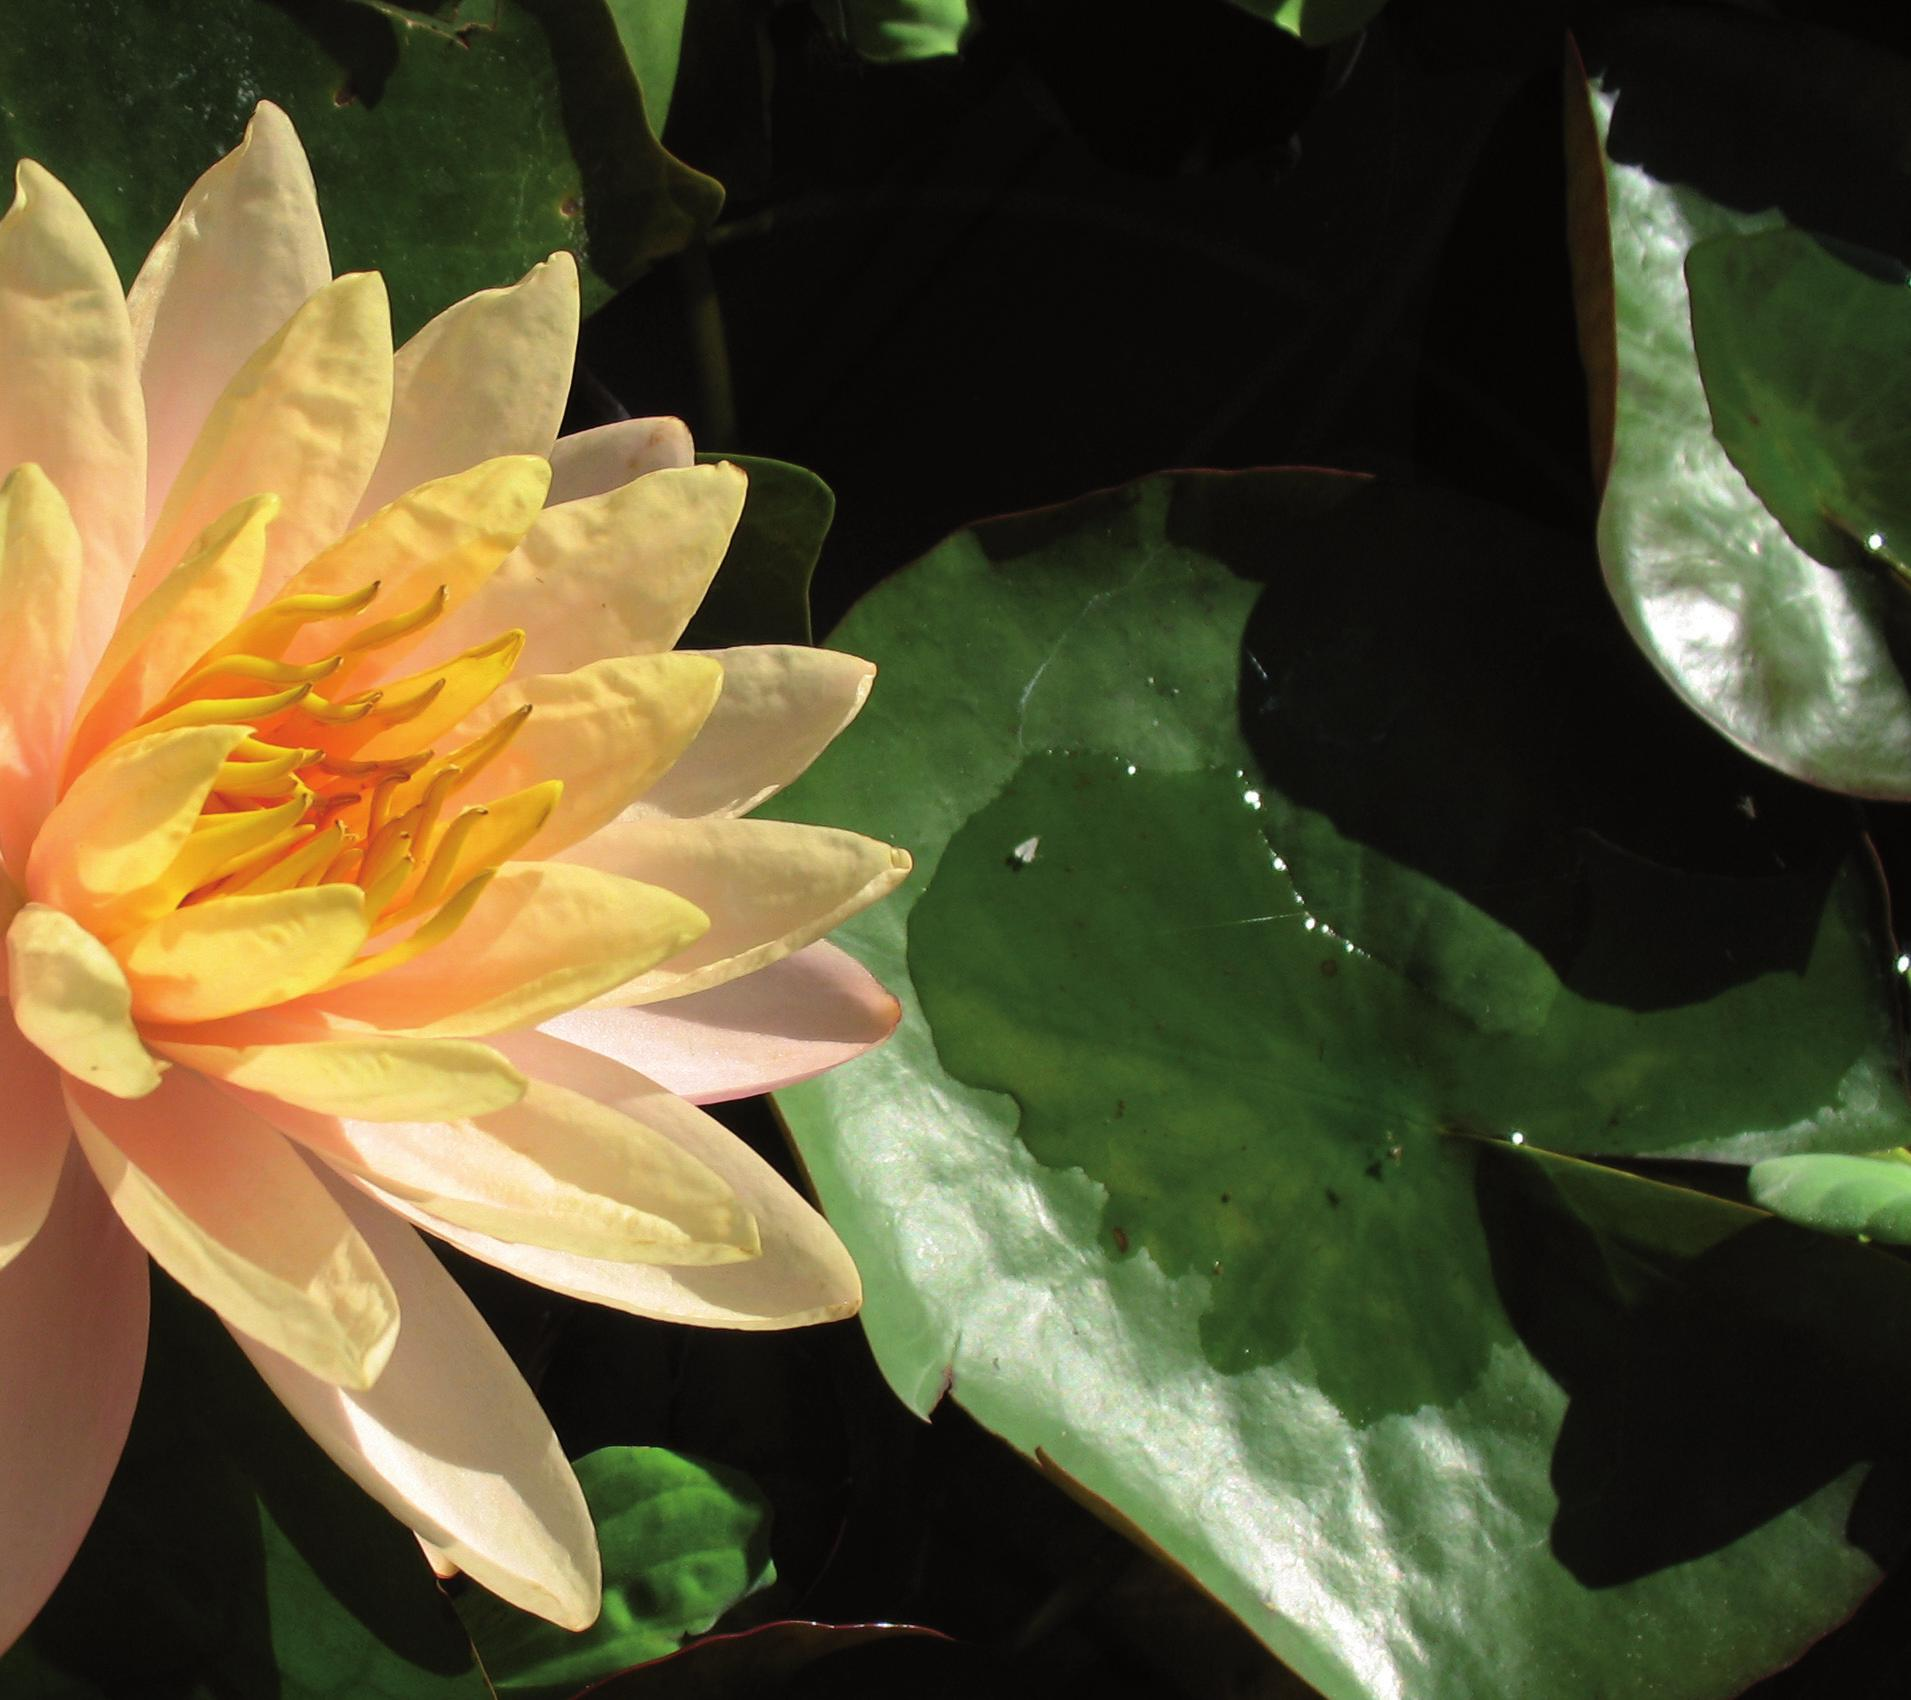
\includegraphics[
  keepaspectratio,
  height={\onePageHeight+4mm},
  clip,
  trim=0 0 18mm 18mm,
]{front-cover-bg.jpg}}}

\raggedleft
\color{white}

{\scshape\LARGE
Ajahn Chah's\\[2mm]
\huge
Teachings On Nature}

\vfill

{\authorFont\Large
by\\
Pasanno Bhikkhu}

\end{document}

